\part{Описание текстового синтаксиса с помощью \tool{Grammatic}}

Что и зачем

\chapter{Мотивация}

Большинство инструментов, автоматизирующих разработку текстового синтаксиса, используют контекстно-свободные грамматики, однако каждый из них использует их по-своему. Оставляя за рамками обсуждения различия в правилах записи продукций, рассмотрим содержательные различия выходных языков различных инструментов.

\section{Операторы}

В каноническом виде КСГ строятся с помощью двух операций: $\rightarrow$ для формирования продукции и конкатенация для формирования правой части продукции. В инструментах семейства \tool{Yacc} (например, \cite{???}), порождающих восходящие анализаторы, используются только эти две операции, что отвечает содержанию нотации BNF.

Однако при построении нисходящих анализаторов набор операций часто расширяют, используя нотацию EBNF. Это связано с тем, что конфликты в LL-грамматиках часто можно устранить, если использовать \term{итерацию}, стандартную операцию в языках регулярных выражений, часто обозначаемую ``*'' (альтернативное обозначение --- фигурные скобки ``\{\ldots\}''). Выражение $A^*$ означает, что цепочка $A$ может повторяться ноль или более раз. Также используют другие операции, применяемые в регулярных выражениях:
\begin{itemize}
\item $A^+$ --- повторение один или более раз;
\item $A^?$ --- вхождение ноль или один раз (альтернативное обозначение --- $[A]$);
\item $A\,|\,B$ --- вхождение $A$ или $B$.
\end{itemize}
Использование этих операций позволяет избежать большинства типичных проблем при разработке LL-грамматик \cite{???}. Разные инструменты поддерживают дополнительные операции в разной степени: так, например, \tool{SableCC} \cite{???} разрешает применять их только на верхнем уровне, и итерировать только одиночные символы.

\section{Описание лексических анализаторов}

При классическом подходе к построению трансляторов \cite{???} фазы лексического и синтаксического анализа описываются отдельно друг от друга. Так, многие известные инструменты состоят из двух (независимых) программ: генераторов лексических и синтаксических анализаторов (\tool{Lex/Yacc}, \tool{flex/Bison}, \tool{Alex/Happy} и т.д.). Входные нотации двух генераторов, как правило, различны, поскольку решают разные задачи. Кроме того, для описания лексических анализаторов чаще всего используются регулярные выражения, имеющие полный набор операций, описанных в предыдущем разделе, а для описания КСГ, как отмечалось выше, часто используется более узкий набор операций.

Однако многие разработанные в последние годы инструменты (например, ANTLR \cite{???}) позволяют описывать лексику и синтаксис языка в одной спецификации (с использованием одних и тех же операций), а некоторые инструменты (например, ASF+SDF \cite{???}) вообще обходятся без фазы лексического анализа, описывая грамматику языка над алфавитом отдельных символов, а не лексем.

\section{Аннотации}

Большинство инструментов не работают с КСГ ``в чистом виде'', а используют нотации, дополняющие грамматики какой-то информацией, например, семантическими продукциями для вычисления атрибутов \cite{???}, типами вершин AST \cite{???}, метками для подвыражений \cite{???}, директивами форматирования \cite{???}, семантическими предикатами \cite{???}, указаниями на семантическую роль терминалов \cite{???} и т.д. Практически каждый инструмент использует грамматики, \term{аннотированные} дополнительной информацией.

\section{Обобщенная нотация}

Нотация языка \tool{Grammatic} призвана обобщить подходы, используемые в других инструментах: она должна позволять описывать как лексическую, так и синтаксическую структуру языка, используя все дополнительные операции EBNF, и снабжать описание аннотациями произвольной сложности. Необходимо, чтобы входной формат любого другого инструмента можно было бы преобразовать в формат \tool{Grammatic} так, чтобы и обратное преобразование было возможно. Таким образом, \tool{Grammatic} становится ``общим знаменателем'' для нотаций, использующих КСГ. Кроме того, нашей целью является реализация механизмов композиции, о которых говорилось в предыдущей главе.

Единственной известной нам попыткой разработки обобщенного формата для представления грамматик, полученных из различных источников, является BGF \cite{ZaitsevLaemmel}. Этот формат поддерживает все операции EBNF, но никак не обрабатывает аннотации и не поддерживает механизмов композиции.

\section{Сценарии использования \tool{Grammatic}}

Наличие обобщенной нотации позволяет использовать \tool{Grammatic} как универсальный инструмент для разработки языков, основанный на принципах \term{порождающего программирования} \cite{???}. Библиотека, поддерживающая обобщенную нотацию, о которой говорилось выше, позволяет преобразовывать аннотированную грамматику во внутреннее структурированное представление (в виде модели), которое может быть подано на вход различных генераторам. 

// Схема грамматика + метаданные --генератор--> код

// Пример про ANTLR

Как показывает практика использования \tool{Grammatic}, этот инструмент удобен для решения следующих задач:
\begin{itemize}
\item генерация лексических и синтаксических анализаторов;
\item генерация трансляторов общего назначения, описываемых с помощью АТГ;
\item автоматическое построение классов AST;
\item создание специальных трансляторов: например, для
	\begin{itemize}
		\item автоматического форматирования кода,
		\item подсветки синтаксиса,
		\item автодополнения в среде разработки;
	\end{itemize}
\item генерация документации;
\item анализ и преобразование грамматик.
\end{itemize}

Примеры применения \tool{Grammatic} для этих задач мы приводим ниже.

\chapter{Основные конструкции языка}

Язык \tool{Grammatic} описывается мета-моделью, приведенной в Приложении \bad{???}. В данном разделе мы описываем конструкции ядра \tool{Grammatic}.

\section{Синтаксические правила}

Структура языка соответствует стандартному определению КСГ (\figref{GCore}): \term{грамматика} представляет из себя набор \term{символов}, каждый из которых определяется одной или несколькими \term{продукциями}. В правой части продукций стоят \term{выражения}, построенные с помощью операций EBNF из символов данной грамматики и \term{терминальных определений}.

\begin{figure}[htbp]
\caption{Основные элементы мета-модели \tool{Grammatic}}\label{GCore}
\end{figure}

Нотация, используемая в \tool{Grammatic} для записи правил КСГ основана на нотации популярного генератора ANTLR, но отличается явным выделением продукций и пустого слова. Проиллюстрируем ее использование на примере языка арифметических выражений, заданного продукциями, представленными на рисунке \figref{ArithProd}:
\begin{lstlisting}
	s
		: VAR '=' e
		;
	e
		: e '+' e
		: e '*' e
		: '(' e ')'
		: INT
		: VAR
		;
\end{lstlisting}

\begin{figure}[htbp]
\newcommand{\gp}[2]{#1 & \rightarrow & #2 }
$$
\begin{array}{rcllrcl}
\multicolumn{7}{c}{
	\begin{array}{rcl}
		\gp{S}{\mathbf{var} \, = \, E}\\
	\end{array}
}\\
\gp{E}{E \, \mathbf{+} \, E}&\quad&
\gp{E}{E \, \mathbf{*} \, E}\\
\gp{E}{\mathbf{int}} &&
\gp{E}{\mathbf{var}} \\
\multicolumn{7}{c}{
	\begin{array}{rcl}
		\gp{E}{\mathbf{(} E \mathbf{)}}\\
	\end{array}
}\\
\end{array}
$$
\caption{КС-продукции, описывающие арифметические выражения}\label{ArithProd}
\end{figure}

Как видно из примера, левая и правая части продукции отделяются друг от друга двоеточием, причем символ в левой части пишется один раз для всех продукций. В данном примере определяются только ``синтаксические правила'' \code{s} и \code{e}. В принципе, символы \code{INT} и \code{VAR} ничем не отличаются с точки зрения нотации, однако при традиционном подходе эти символы были бы терминальными. \tool{Grammatic} не разделяет символы на терминалы и нетерминалы, поскольку, как говорилось выше, для некоторых алгоритмов разбора это разделение не имеет смысла. Таким образом, все символы в спецификации являются нетерминальными, а терминалы представлены литералами в одинарных кавычках. Несмотря на отсутствие принципиального раздGCoreеления с точки зрения языка, мы придерживаемся обозначений, разделяющих ``разные'' с нашей точки зрения типы символов: имена терминалов мы пишем заглавными буквами, а нетерминалов --- начиная со строчной буквы\footnote{Этот способ именования также позаимствован из языка спецификаций ANTLR, в котором он является обязательным.}.

Определения символов \code{INT} и \code{VAR} выглядят так:
\begin{lstlisting}
	INT : DIGIT+;
	VAR : IDEN_START IDEN_PART*;
	DIGIT : ['0'--'9'];
	IDEN_START : ['a'--'z''A'--'Z''_'];
	IDEN_PAR : digit | idenStart;
\end{lstlisting}
Этот пример иллюстрирует использование различных элементов нотации \tool{Grammatic}. Полный перечень представлен в \tabref{operations}.
\begin{figure}[htbp]
\center
	\begin{tabular}{|c|l|}
	\hline
	\bf Нотация & \bf Значение \\
	\hline
	\code{\#empty} & Пустое выражение \\
	\code{a} & Ссылка на символ a \\
	\code{a b} & Последовательность \\
	\code{a | b} & Альтернатива \\
	\code{a*} & Итерация от 0 до бесконечности \\
	\code{a+} & Итерация от 1 до бесконечности \\
	\code{a?} & Итерация от 0 до 1 \\
	\code{['a'--'z']} & Множество символов от 'a' до 'z' \\
	\code{'abc'} & Строка символов 'abc' \\
	\code{(a | b) c} & Круглые скобки для группировки выражений \\
	\hline
	\end{tabular}
	\caption{Выражения \tool{Grammatic}}\label{operations}
\end{figure}
Еще одним хорошим примером послужит описание нотации \tool{Grammatic} с помощью нее самой, приведенное в Приложении \bad{???}.

// Приоритеты бинарных операций

\section{Метаданные}

Метаданными называют описательные элементы программ, которые не обрабатываются компилятором, но и не являются комментариями: к ним могут получить доступ дополнительные инструменты, работающие с кодом. По аналогии с \tool{Java} метаданные поддерживаются и в \tool{Ecore}: каждому элементу мета-модели можно сопоставить произвольное количество \tool{аннотаций}. В следствие сходства с этими подходами, мы тоже называет аннотации в \tool{Grammatic} метаданными.

Как отмечалось выше, для решения различных задач грамматики необходимо снабжать аннотациями, которые будут позже использоваться генераторами. Типичным примером аннотаций являются семантические действия, но это далеко не единственный пример. Так, для построения программы-форматировщика, добавляющей в текст пробелы и переводы строк для того, чтобы текст выглядел ``структурно'', правила форматирования также задаются в виде аннотаций к грамматике, но не содержат инструкций для вычисления каких-либо атрибутов (подробно эта задача будет рассмотрена ниже в этой главе). То же касается и многих других типичных задач, связанных с созданием интегрированных сред разработки: подсветкой синтаксиса, сворачиванием блоков, построением визуального представления структуры программы и т.д. Заранее предвидеть все возможные применения системы нельзя, поэтому \tool{Grammatic} предоставляет гибкий механизм для описания аннотаций произвольной сложности.

Аннотации могут быть присоединены к любому элементу грамматики: символу, продукции, выражению или всей грамматике целиком. Каждая аннотация представляет из себя набор пар ``имя-значение''. В текстовом синтаксисе это оформляется с помощью фигурных скобок:
\begin{lstlisting}
	s{a = 10} 
		: {b = 'abc'} 
		  (e{c = asd})* { d = {x = 5; y = 6} };	
\end{lstlisting}
Пары ``\tool{имя = значение}'' мы будем называть \term{атрибутами}\footnote{Использование этого термина может вызвать путаницу с атрибутами в АТГ, но в нашем обсуждении из контекста всегда будет понятно, о каких атрибутах идет речь.}. В приведенном примере 
\begin{itemize}
\item атрибут \code{a} сопоставлен с символом \code{s} и имеет значение \code{10} (целое число); 
\item атрибут \code{b} сопоставлен с продукцией (такие аннотации пишутся сразу после двоеточия, начинающего продукцию) и имеет значение \code{'abc'} (строка);
\item атрибут \code{с} сопоставлен с вхождением символа \code{e} в правую часть продукции (а не с самим символом!) и имеет значение \code{abc} (идентификатор);
\item атрибут \code{d} сопоставлен с выражением \code{e*} и имеет значение \code{{x = 5; y = 6}} (аннотация, состоящая из двух атрибутов).
\end{itemize}
Предопределенные типы значений, приведенные в \tabref{attr-types}, позволяют создавать довольно сложные аннотации. Наибольшую свободу предоставляет тип ``Последовательность'', значения которого являются последовательностями значений других типов и знаков препинания. Ниже мы увидим, как с помощью таких атрибутов можно создавать небольшие ``предметно-ориентированные языки'' внутри \tool{Grammatic}.
\begin{figure}[htbp]
\center
	\begin{tabular}{|c|l|}
	\hline
	\bf Нотация & \bf Значение \\
	\hline
	\code{'abc'} & Строка \\
	\code{10} & Целое число \\
	\code{abc} & Идентификатор \\
	\code{\{ a = b; c = 10\}} & Аннотация \\
	\code{ \{\{ a, b, c ; \}\} } & Последовательность \\
	\code{ << s | (a b)* >> } & Грамматическое выражение \\
	\hline
	\end{tabular}
	\caption{Предопределенные типы значений атрибутов}\label{operations}
\end{figure}
Однако для некоторых целей предопределенных типов не хватает. В этом случае можно определять пользовательские типы значений, что достигается расширением иерархии классов мета-модели (см. Приложение \bad{???}).

В некоторых случаях атрибут играет роль флага: его значение не важно, а роль играет только наличие или отсутствие атрибута. В таких случаях значение атрибута можно не указывать: указывается только имя (без знака равенства). Например, при генерации трансляторов удобно помечать некоторые символы грамматики (как правило ``терминальные'') как элементы форматирования (whitespace) --- чтобы анализатор их игнорировал. Это актуально не только для настоящих символов форматирования (пробелов, переводов строк, табуляции), но и для комментариев. Для такой реализации пометки достаточно указать атрибут без значения:
\begin{lstlisting}
	WS{ignore} : [0x0000-0x0020];
\end{lstlisting}
Заметим, что имя атрибута, которое нужно указать, зависит от конкретного генератора, для которого пишется спецификация. Семантика языка \tool{Grammatic} никак не интерпретирует атрибуты.

Поскольку в одной грамматике могут встречаться атрибуты, предназначенные для разных генераторов, необходимо обеспечить уникальность имен, чтобы атрибуты не ``накладывались''. Это достигается с помощью введения \term{пространств имен} для атрибутов. Пространство имен идентифицируется однородным идентификатором ресурса (Uniform Resource Identifier, URI \cite{???}), внутри данной грамматики для удобства ему присваивается локальное имя, это делается с помощью директивы \code{namespace}:
\begin{lstlisting}
	namespace example 'http://example.com/Namespace/Example';
\end{lstlisting}
Для нужд самого \tool{Grammatic} выделено системное пространство имен \code{system} с URI \code{grammatic:/}. По умолчанию все атрибуты определяются в системном пространстве имен. Чтобы указать другое пространство имен, используется квалифицированное имя атрибута, например:
\begin{lstlisting}
	A{example.size = 10}
\end{lstlisting}
Различные генераторы должны определять свои пространства имен, чтобы избегать наложения атрибутов.

\section{Пример: интерпретатор арифметических выражений}

показать примеры аннотаций: ATG/SDT, ASF+SDF, Bison, Pretzel, xText

\begin{lstlisting}
	WS{ignore} : [0x0000-0x0020];
	COMMENT{ignore} : '//' [^'\n']*;
	DIGIT{lexical; fragment} : ['0'--'9'];
	IDEN_START{lexical; fragment} : ['a'--'z''A'--'Z''_'];
	IDEN_PAR{lexical; fragment} : digit | idenStart;
	VAR{lexical} : IDEN_START IDEN_PART*;
	INT{lexical} : DIGIT+;
\end{lstlisting}

\begin{lstlisting}
{
	priorities = {{ '+' < '*' }};
}
\end{lstlisting}

\begin{lstlisting}
	e{returns=int} 
		: e{assignTo=a} '+' e{assignTo=b; code='result = a + b;'}
		: e{assignTo=a} '*' e{assignTo=b; code='result = a * b;'}
		: INT{assignTo=a; code='result = stringToInt(a);'}
		: '(' e{assignTo=a; code='result = a;'} ')'
		;
\end{lstlisting}

\begin{lstlisting}
	s
		: { scope = {{ put(s.scope, VAR, e.value) }} }
		VAR '=' e
		;
	e
		: { value = {{ e[1].value + e[2].value }} }
		  e '+' e
		: { value = {{ e[1].value * e[2].value }} }
		  e '*' e
		: { value = {{ stringToInt(INT) }} }
		  INT
		: { value = {{ get(s[].scope, VAR) }} }
		  VAR
		: { value = {{ e[1] }} }
		  '(' e ')'
		;
\end{lstlisting}

\section{Пример: язык для описания конечных автоматов}

Для демонстрации возможностей \tool{Grammatic} ниже мы будем использовать предметно-ориентированный язык StateMachine, предложенный М. Фаулером \cite{???} и широко используемый в литературе по ПОЯ \cite{???}. В данном разделе мы приводим неформальное описание этого языка, дающее представление о его назначении и содержании.

Язык StateMachine позволяет описывать простые конечные автоматы Мура \cite{???}, то есть автоматы, допускающие только действиями в состояниях, но не на переходах. Целевая мета-модель этого языка представлена на \figref{SMMM}.

\begin{figure}[htbp]
	\caption{Целевая мета-модель языка StateMachine}\label{SMMM}
\end{figure}

В графической состояния изображаются вершинами графа, переходы --- направленными ребрами (см. \figref{SM}). В вершинах над горизонтальной чертой пишется уникальный идентификатор состояния, а под чертой --- выходные воздействия, генерируемые в этом состоянии. На переходах пишутся входные воздействия, их инициирующие.

\begin{figure}[htbp]
	\centering
	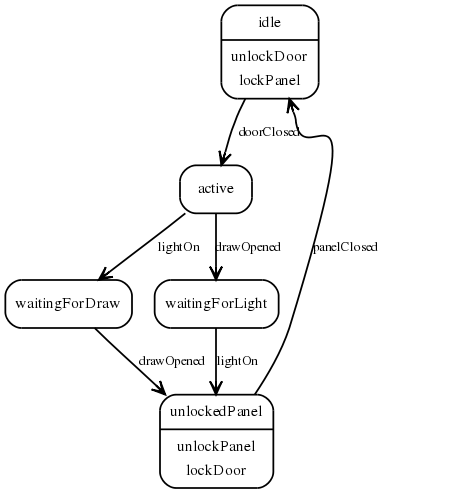
\includegraphics[scale=.7]{smgraph.png}
	\caption{Графическая нотация для языка StateMachine (из \cite{???})}\label{SM}
\end{figure}

В текстовой нотации автомат описывается с помощью ключевого слова \code{statemachine}, за которым следуем имя автомата и набор состояний в фигурных скобках. Пример использования текстовой нотации приведен в \lstref{SMText}. Cостояния описываются с помощью ключевого слова \code{state}; внутри состояния может находиться блок \code{do}, содержащий последовательность выходных воздействий, а также переходы, описываемые с помощью конструкции \code{on INPUT goto STATE}, где \code{INPUT} --- входное воздействие, а \code{STATE} --- состояние, в которое осуществляется переход.

Входные и выходные воздействия описываются вне блока \code{statemachine} с помощью ключевого слова \code{event}; каждое воздействие имеет уникальное имя и целочисленный код.

\begin{lstlisting}[label=SMText,float=htbp,caption=Текстовая нотация языка StateMachine]
event lockDoor 0; event unlockDoor 1;
event lockPanel 2; event unlockPanel 3;
event doorClosed 4; event doorOpened 5;
event lightOn 6; event drawOpened 7;
event panelClosed 8;

statemachine SecretCompartment {
	state idle {
		do {
			unlockDoor;
			lockPanel;
		}
		on doorClosed goto active;
	}
	state active {
		on lightOn goto waitingForDraw;
		on drawOpened goto waitingForLight;
	}
	state waitingForDraw {
		on drawOpened goto unlockedPanel;
	}
	state waitingForLight {
		on lightOn goto unlockedPanel;
	}
	state unlockedPanel {
		do {
			unlockPanel;
			lockDoor;
		}
		on panelClosed goto idle;
	}
}
\end{lstlisting}

Синтаксические правила языка StateMachine, выраженные в нотации \tool{Grammatic}, приведены в \lstref{SMGram}.

\begin{lstlisting}[xleftmargin=1cm,label=SMGram,caption=Грамматика языка StateMachine]
WS : [0x0000-0x0020];
COMMENT : '//' [^'\n']*;
DIGIT : ['0'-'9'];
NAME_START : ['a'-'z''A'-'Z'_];
NAME_PART : NAME_START | DIGIT;
NAME : NAME_START NAME_PART*;
INT : DIGIT*;

system : event* stateMachine;
stateMachine : 'statemachine' NAME '{' state* '}';
state : 'state' NAME '{' do? (transition ';')* '}';
do : 'do' block;
transition : 'on' eventRef 'goto' stateRef;
stateRef : NAME;
block : '{' (commandRef ';')* '}';
eventRef : NAME;
commandRef : NAME;
event : 'event' NAME INT;
\end{lstlisting}

\chapter{Модули}

Поддержка модулей позволяет разработчику разделять спецификацию на несколько отдельных файлов и при необходимости использовать определения из одного файла повторно.  С точки зрения целевой мета-модели \tool{Grammatic}, модулю соответствует грамматика, определенная в отдельном файле. В данном разделе мы подробно опишем механизм работы таких модулей.

\section{Цитирование и переименование}

Для описания модулей в \tool{Grammatic} не применяется никаких специальных синтаксических конструкций, поэтому файл, содержащий описание грамматики, уже является модулем. Для того, чтобы использовать один модуль внутри другого, применяется директива цитирования \tool{import}, синтаксис которого можно проиллюстрировать на следующем примере:
\begin{lstlisting}
import 'a/b/c/d.grammar' {A, B as C};

B : A C*;
\end{lstlisting}  
Директива \code{import} принимает два аргумента: идентификатор импортируемого файла в одинарных кавычках и список импортируемых символов в фигурных скобках. 

Идентификатором файла является его имя в \term{виртуальной файловой системе}, конфигурация которой подается на вход транслятору \tool{Grammatic} вместе с файлом основной грамматики. В простейшем случае (пустая конфигурация) виртуальная файловая система в точности соответствует физической, и идентификатором файла является просто путь на диске. Однако при использовании библиотек привязка к путям в физической файловой системе приводит к трудностям с переносимостью, поэтому виртуальная файловая система может предоставлять абстрактное представление физической, самостоятельно находя библиотечные модули. Подробнее формат описания виртуальной файловой системы разобран в Приложении \bad{???}.

Список импортированных символов указывается явно для того, чтобы подчеркнуть характер зависимости данного модуля от подключаемого. При необходимости импортировать все символы, список можно заменить знаком \code{\{*\}}.

Ключевое слово \code{as} используется в случае необходимости импортировать символ под другим именем. Так в нашем примере символ \code{B} переименовать необходимо, поскольку в импортирующем модуле определен символ с таким именем. В результате, правило, описанное здесь соответствует диаграмме на \figref{GRenaming}.

\begin{figure}[htbp]
	\caption{Иллюстрация результата переименования}\label{GRenaming}
\end{figure}

Другая форма директивы цитирования позволяет назначить имя самому импортируемому модулю и обращаться к его элементом с помощью квалифицированных имен:
\begin{lstlisting}
import 'a/b/c/d.grammar' as D;

B : D.A D.B*;
\end{lstlisting}  
Заметим, что при трансляции данного примера результат будет идентичным предыдущему, поскольку в правиле для символа \code{B} мы использовали те же символы из подключаемого модуля (\code{A} и \code{B}) в тех же позициях.

\section{Атрибуты доступа}

Нотация \tool{Grammatic} не предусматривает специальных средств для обозначения атрибутов доступа для правил. Тем не менее, соответствующую функциональность обеспечивают специальные атрибуты \code{private} и \code{public}, зарезервированные для этих целей в системном пространстве имен.

\tool{Grammatic} проверяет наличие атрибута \code{private}, и если он есть, запрещает импортировать символ или использовать его квалифицированное имя. Атрибут \code{public} определен для симметрии, и его можно не указывать. Так, в следующем примере недоступен другим модулям только символ \code{C}:
\begin{lstlisting}
A{public} : B C;
B : C;
C{private} : 'c'
\end{lstlisting}  

\section{Модульная грамматика для языка StateMachine}\label{ModularSMG}

В качестве примера, разделим на модули грамматику языка StateMachine, приведенную в \lstref{SMGram}. Первый модуль \code{smlexer.grammar} будет содержать ``лексические'' определения, которые будут использованы в других модулях:
\begin{lstlisting}
// smlexer.grammar
WS{private} : [0x0000-0x0020];
COMMENT{private} : '//' [^'\n']*;
DIGIT{private} : ['0'-'9'];
NAME_START{private} : ['a'-'z''A'-'Z'_];
NAME_PART{private} : NAME_START | DIGIT;
NAME : NAME_START NAME_PART*;
INT : DIGIT*;
\end{lstlisting}
Заметим, что доступными извне являются только символы \code{INT} и \code{NAME}, поскольку все остальные символы носят служебный характер.

Основные синтаксические правила мы разделим на два модуля: \code{smmain.grammar}, определяющий структуру автомата, и \code{smevents.grammar}, описывающий входные и выходные воздействия:
\begin{lstlisting}
// smmain.grammar

import 
	'smlexer.grammar' {NAME},
	'smevents.grammar' {*};

system : event* stateMachine;
stateMachine : 'statemachine' NAME '{' state* '}';
state : 'state' NAME '{' do? (transition ';')* '}';
do : 'do' block;
transition : 'on' eventRef 'goto' stateRef;
stateRef : NAME;
block : '{' (commandRef ';')* '}';

// smevents.grammar
import 
	'smlexer.grammar' {NAME, INT};
	
eventRef : NAME;
commandRef : NAME;
event : 'event' NAME INT;
\end{lstlisting}
Данный пример демонстрирует возможность повторного использования модуля \code{smlexer.grammar}.

\chapter{Шаблоны}

Как отмечалось выше, шаблоны (макроопределения) позволяют повторно использовать фрагменты грамматики, внося в них некоторые изменения, посредством подстановки на место параметров шаблона реальных значений. Например, если в нотации языка StateMachine мы бы хотели сделать последнюю точку с запятой в списках выходных воздействий и переходов необязательной (как в языке Pascal), нам пришлось бы дважды написать относительно запутанное выражение:
\begin{lstlisting}
state : 'state' NAME '{' do? 
			(transition (';' transition)* ';'?)* 
		'}';
block : '{' 
			(commandRef (';' commandRef)* ';'?)* 
		'}';
\end{lstlisting}

В грамматиках больш\'{и}х языков повторения подобных конструкций могут встречаться десятки раз. Чтобы избежать дублирования, можно определить шаблон вида ``\code{элемент~(разделитель~элемент)*~разделитель?}'', и применить его дважды, подставляя разные значения вместо параметров ``\code{разделитель}'' и ``\code{элемент}'', что позволяет сократить длину кода, улучшить его читаемость и уменьшить вероятность появления ошибок.

В нотации \tool{Grammatic} шаблоны объявляются следующим образом:
\begin{lstlisting}
template List<element : Expression, sep : Expression> : Expression {
	<element> (<sep> <element>)* <sep>?
}
\end{lstlisting}
Первая строка определяет \term{сигнатуру шаблона}, как мы покажем ниже, она используется для гарантий структурной корректности результатов применения шаблона. После двоеточия указывается тип параметра (или результата). Типы соответствуют классам мета-модели \code{Grammatic} (см. \figref{GCore}). Часто (в частности, в данном примере) типы можно опускать, поскольку транслятор способен определить их самостоятельно. В целом, шаблон напоминает функцию: у него есть имя, аргументы и возвращаемое значение; единственное отличие состоит в том, что при применении шаблона результат вычисляется транслятором статически, а не ``во время выполнения''\footnote{Что такое ``время выполнения'' для языка \code{Grammatic} не вполне ясно, тем не менее, что понятие ``статическиого вычисления'' не вызывает сомнений: такие вычисления выполняются транслятором в процессе вычисления функции $Meaning$.}. Аналогично функциям, чтобы использовать ранее определенный шаблон, нужно указать его имя и параметры:
\begin{lstlisting}
state : 'state' NAME '{' do? 
			<List transition, ';'>
		'}';
block : '{' 
			<List commandRef, ';'>
		'}';
\end{lstlisting}
Содержание этого определения символов \code{state} и \code{block} идентично приведенному выше.

Теперь приступим к более детальному описанию механизма шаблонов в \tool{Grammatic}.

\section{Элементы языка шаблонов}
Целевая мета-модель, описывающая шаблоны, приведена на \figref{TempMM}.

\begin{figure}[htbp]
	\centering
	\caption{Целевая мета-модель языка шаблонов}\label{TempMM}
\end{figure}

Выше было показано, что шаблоны реализуются как инфраструктурная функциональность. Это означает, что, добавляя шаблоны в язык, мы расширяем основную нотацию, добавляя новые конструкции так, чтобы получившуюся нотацию можно было транслировать в исходную. Можно считать, что мы создаем новый язык: на основе уже описанного языка грамматик строим языка шаблонов грамматик.

В этом новом языке центральным понятием является \term{шаблонное выражение}: то, что может являться телом шаблона. На \figref{TempMM} шаблонным выражениям соответствуют классы-наследники TemplateExpression. Простейшие шаблонные выражения --- это константы, то есть обычные выражения языка описания грамматик, не содержащие шаблонных параметров и обращений к шаблонам. Например, выражение \code{A B* | C}, как и все его подвыражения, является примером такой константы. Таким образом, нотация для шаблонных выражений включает в себя нотацию для грамматик как подмножество. Заметим, что шаблонные выражения имеют типы, соответствующие классам в целевой мета-модели языка грамматик.

Новыми элементами в нотации шаблонных выражений являются обращения к шаблонным параметрам (класс ParameterUsage), которые записываются в угловых скобках (\code{A <paramName>* | C}), и вызовы шаблонов (класс TemplateApplication), которые также заключаются в угловые скобки, но, кроме имени, содержат также список аргументов шаблона, разделенных запятыми:
\begin{lstlisting}
	<List expression, ';'>
\end{lstlisting}
Заметим, что, если шаблон не имеет параметров (то есть является константным), вызов такого шаблона синтаксически неотличим от обращения к параметру, что выражает близость этих двух понятий.

Шаблонные выражения записываются внутри объявлений шаблонов (класс Template), и представляют собой \term{тело} шаблона. Синтаксически объявление шаблона оформляется с помощью ключевого слова \code{template}:
\begin{lstlisting}
template List<element : Expression, sep : Expression> : Expression {
	<element> (<sep> <element>)* <sep>?
}
\end{lstlisting}
Как мы отмечали выше, типы, указанные в объявлении, используются для гарантий корректности результата применения данного шаблона. Шаблонные параметры, описанные в сигнатуре шаблона, могут быть использованы только в его теле. Объявления шаблонов не вкладываются одно в другое, также не допускаются рекурсивные вызовы шаблонов (прямые или косвенные), поскольку вычисление значения при вызове такого шаблона никогда не закончится.

Типы, используемые при объявлении шаблонов строятся по следующим правилам: 
\begin{itemize}
\item \term{Элементарные типы} --- это классы мета-модели грамматик (Expression, Sequence, Production, Symbol и т.д.).
\item \term{Составные типы} образуются из элементарных следующими операциями:
	\begin{itemize}
		\item ``?'' значение элементарного типа является необязательным;
		\item ``+'' непустой список значений элементарного типа;
		\item ``*'' произвольный список значений элементарного типа.
	\end{itemize}
\end{itemize}

\section{Примеры использования шаблонов}

Выше мы показали, как и для чего могут быть использованы шаблоны отдельных выражений. Для таких целей шаблоны применяются в EBNF \cite{???} и \tool{Menhir} \cite{???}. В Главе \ref{part1} мы также описывали параметризованные модули, используемые в \tool{ASF+SDF} и \tool{Rats!}, в данном разделе мы покажем, как шаблоны \tool{Grammatic} позволяют реализовать аналогичную функциональность. Кроме того, мы покажем, что можно использовать и шаблоны метаданных.

\subsection{Параметризованные модули}

Мы разработаем вариант описания языка StateMachine, который позволит нам варьировать содержание понятий входного и выходного воздействия. В разделе \ref{ModularSMG} мы выделили три модуля в грамматике языка StateMachine, один из которых, \code{smevents.gramar} содержал определения для символов \code{even}, \code{eventRef} и \code{commandRef}, которые использовались в главном модуле. Такая реализация уже позволяет изменять определения данных символов, не изменяя кода главного модуля, но она не позволяет использовать \term{параллельно} два варианта реализации понятия ``воздействие''. Для того, чтобы поддержать эту возможность, мы видоизменим главный модуль, введя шаблонные параметры:
\begin{lstlisting}
// smmain.grammar

import 
	'smlexer.grammar' {NAME};

template SMMain<event : Expression, eventRef : Expression, 
		commandRef : Expression> : Symbol+ 
{
	system : <event>* stateMachine;
	stateMachine : 'statemachine' NAME '{' state* '}';
	state : 'state' NAME '{' do? (transition ';')* '}';
	do : 'do' block;
	transition : 'on' <eventRef> 'goto' stateRef;
	stateRef : NAME;
	block : '{' (<commandRef> ';')* '}';
}
\end{lstlisting}
Важно заметить, что модуль \code{smevents.grammar} больше не используется, а вместо обращений к символам этого модуля введены шаблонные параметры.

Теперь определим два сосуществующих варианта описания входных и выходных воздействий: первый --- тот, что уже использовался, а второй --- позволяющий сопоставить каждому воздействию строку для записи в журнал событий. Первый вариант реализует уже знакомый нам модуль \code{smevents.grammar}:
\begin{lstlisting}
// smevents.grammar
import 
	'smlexer.grammar' {NAME, INT};
	
eventRef : NAME;
commandRef : NAME;
event : 'event' NAME INT;
\end{lstlisting}
Второй вариант мы реализуем в модуле \code{smevents-log.grammar}:
\begin{lstlisting}
// smevents-log.grammar
import 
	'smlexer.grammar' {NAME, INT};
	
logEventRef : NAME;
logCommandRef : NAME;
logEvent : 'event' NAME INT STRING?;

STRING : '\'' [^'\'''\n''\r']* '\'';
\end{lstlisting}

Теперь необходимо соединить каждую из этих реализаций с главным модулем. Для этого достаточно применить определенный этим модулем шаблон и передать соответствующие параметры. Для первого случая получим
\begin{lstlisting}
<SMMain event, eventRef, commandRef>
\end{lstlisting}
Для второго случая получим
\begin{lstlisting}
<SMMain logEvent, logEventRef, logCommandRef>
\end{lstlisting}
Шаблоны делают данные определения гораздо компактнее: если бы нам пришлось обходиться обычными модулями, определение главного модуля пришлось бы записать дважды --- по одному разу для каждого варианта реализации воздействий.

// Параметризация грамматики другими грамматиками

// импортирование vs встраивание

\subsection{Шаблоны метаданных}

Поскольку метаданные тоже входят в основную нотацию \tool{Grammatic}, можно создавать и шаблоны аннотаций. В основном, такие шаблоны понадобятся нам для реализации механизма аспектов, а в этом разделе мы приведем простой пример, показывающий, как с их помощью можно регламентировать структуру аннотаций.

Генератор документации для грамматик использует метаданные как источник дополнительной информации: специальные атрибуты хранят текст, описывающий назначение символа, примеры строк, которые он выводит и т.д. Для примера приведем описание оператора \code{if} некоторого гипотетического языка:
\begin{lstlisting}
if
{	doc.title = 'Conditional operator';
	doc.description = 
'If expression evaluates to true, <code>then</code> branch is taken,
otherwise -- <code>else</code> branch is taken';
	doc.examples = {{
		'if a > 1 then WriteLn(a)'
		'if (x < 0) and (x > -5) then x := -x else x := 2 * x'
	}}
} : 'if' expression 'then' statement ('else' statement) ;
\end{lstlisting}

Из такого описания генератор построит следующий текст:
\begin{center}
\fbox{
\parbox{0.7\textwidth}{
{{\bf Conditional operator}\\
\small
{\bf Syntax}: \\
\textit{if} ::= \texttt{if} \textit{expression} \texttt{then} \textit{statement} \texttt{else} \textit{statement}\\
{\bf Description}: 
If expression evaluates to true, \texttt{then} branch is taken,
otherwise -- \texttt{else} branch is taken\\
{\bf Examples}: 
\begin{itemize}
\item \textbf{if} a > 1 \textbf{then} WriteLn(a)
\item \textbf{if} (x < 0) \textbf{and} (x > -5) \textbf{then} x := -x \textbf{else} x := 2 * x
\end{itemize}
}}}
\end{center}

Мы используем шаблон аннотации для того, чтобы гарантировать, что разработчик укажет все атрибуты, необходимые для генерации документации:
\begin{lstlisting}
template Doc<title : String, description : String, 
	examples : String+> : Attribute+ 
{
	doc.title = <title>;
	doc.description = <description>;
	doc.examples = {{ <examples> }};
}
\end{lstlisting}
С применением этого шаблона метаданные для символа \code{if} будут выглядеть так:
\begin{lstlisting}
if
{Doc<
'Conditional operator',
'If expression evaluates to true, <code>then</code> branch is taken,
otherwise -- <code>else</code> branch is taken',
'if a > 1 then WriteLn(a)',
'if (x < 0) and (x > -5) then x := -x else x := 2 * x'
>} : 'if' expression 'then' statement ('else' statement) ;
\end{lstlisting}
В этом случае \tool{Grammatic} выдаст сообщение об ошибке, если один из элементов документации не будет указан.

\section{Формализация языка шаблонов}

Для того, чтобы описать язык шаблонов более точно, мы приводим в этом разделе формальное описание его контекстно-свободного синтаксиса, системы типов и семантики. Чтобы не загромождать текст разбором однотипных случаев, мы упрощаем формализуемый язык, рассматривая только выражения (опуская определения символов и продукции), а среди них --- только операцию конкатенации и строковые литералы. Более полное описание вынесено в Приложение \bad{???}.

Контекстно-свободная грамматика упрощенного языка шаблонов приведена в \lstref{TempG}. В этой грамматике упоминаются только типы, соответствующие рассматриваемым нами конструкциям языка (\texttt{Sequence} для конкатенации и \texttt{Literal} для строковых литералов). Аппарат шаблонов описан в полном объеме: объявления и применения шаблонов и использование параметров.

\begin{lstlisting}[float=htbp,label=TempG,caption=Грамматика упрощенного языка шаблонов]
templateDef
	: 'template' NAME '<' 
			List<NAME type?, ','> 
	  	'>' type? '{' expression '}'
	;
type : ':' ('Expression' | 'Literal' | 'Sequence') ;
expression
	: expression expression
	: STRING
	: templateParameterRef
	: templateApplication
	;
templateParameterRef : '<' NAME '>'	;
templateApplication	: '<' NAME List<expression, ','> '>' ;
\end{lstlisting}

Для того, чтобы гарантировать, что результат применения шаблона будет корректным с точки зрения целевой мета-модели, мы определяем систему типов для языка шаблонов. Правила этой системы типов приведены на \figref{TempTypes}. Требования целевой мета-модели моделируются с помощью отношения ``подтип'', обозначаемого следующим образом:
$$
	\mbox{подтип} \preceq \mbox{супертип}.
$$
В остальном система типов выражена традиционным способом (см. \cite{???}). Слева от символа выводимости $\vdash$ пишется \term{контекст} (чаще всего обозначаемый $\Gamma$. В нашем случае контекст представляет собой множество утверждений вида $e : \tau$, где $e$ --- шаблонное выражение, а $\tau$ --- тип; такие утверждения читаются как ``\term{$e$ имеет тип $\tau$}''. 

\newcommand{\trule}[3]{%
\dfrac{#1}{#2}(\mbox{\textsc{#3}})%
}%
%
\begin{figure}[htbp]
$$
\begin{array}{ccc}
\trule{}{\mathtt{Literal} \preceq \mathtt{Expression}}{lit-sub}
&&
\trule{}{\mathtt{Sequence} \preceq \mathtt{Expression}}{seq-sub}
\\
&&\,\\
\trule{}{STRING : \mathtt{Literal}}{lit-t}
&\quad&
\trule{}{\Gamma \cup \{p : \tau\} \vdash <p> : \tau}{par-t}
\\
&&\,\\
%
\trule{
	\Gamma \vdash e_1 : \mathtt{Expression} 
	\quad 
	\Gamma \vdash e_2 : \mathtt{Expression}
}{
	\Gamma \vdash e_1 \, e_2 : \mathtt{Sequence}
}{seq-t}
&&
\trule{
	\Gamma \vdash e : \tau
	\quad 
	\tau \preceq \sigma 
}{
	\Gamma \vdash e : \sigma
}{subtype}
\\
&&\,\\
\multicolumn{3}{c}{
\trule{
	\Gamma \cup \bigcup\limits_{i=1}^{n} \{ p_i : \tau_i \} \vdash b : \sigma
}{
	\Gamma \vdash \mathbf{template}\left(
		T <p_1 : \tau_1, \ldots, p_n : \tau_n> \,: \sigma \, \{ b \}
	\right)
}{temp-def}
}
\\
&&\,\\
\multicolumn{3}{c}{
\trule{
	\Gamma \vdash \mathbf{template}\left(
		T <p_1 : \tau_1, \ldots, p_n : \tau_n> \,: \sigma \, \{ b \}
	\right)
	\quad
	\Gamma \vdash a_1 : \tau_1 \, \cdots \, \Gamma \vdash a_n : \tau_n
}{
	\Gamma \vdash <T \, a_1, \ldots, a_n> : \sigma
}{app-t}
}
\end{array}
$$
	\caption{Система типов упрощенного языка шаблонов}\label{TempTypes}
\end{figure}

\newcommand{\Inst}[2]{\mathcal{I}_{#1} \left[ #2 \right]}%
Семантика языка шаблонов задается операцией \term{разворачивания}, описанной в композиционном стиле правилами на \figref{TempSem}. Мы обозначаем результат разворачивания шаблонов в выражении $e$ как $\Inst{\gamma}{e}$, где $\gamma$ (``\term{среда}'') является множеством значений параметров шаблонов вида $p = e$, где $p$ --- параметр, а $e$ --- шаблонное выражение. Как видно из правила \textsc{APP}, когда разворачивается применение шаблона, среда пополняется информацией о текущих значениях параметров, при этом само значение не разворачивается до тех пор, пока оно не будет использовано. Разворачивание значений использованных параметров выполняется в правиле \textsc{PAR}.

\begin{figure}[htbp]
$$
\begin{array}{ccc}
\trule{}{\Inst{\gamma}{STRING} = STRING }{str}
&\quad&
\trule{}{
	\Inst{\gamma}{e_1 \, e_2} = 
		\Inst{\gamma}{e_1} \, \Inst{\gamma}{e_2} 
}{seq}
\\
&&\,\\
\multicolumn{3}{c}{
\trule{
	\{p = e\} \subseteq \gamma
}{
	\Inst{\gamma}{<p>} = \Inst{\gamma}{e}
}{par}
}
\\
&&\,\\
\multicolumn{3}{c}{
\trule{
	\mathbf{template}\left(
		T \, <p_1, \ldots, p_n> \, \{ b \}
	\right)
}{
	\gamma' = \bigcup\limits_{i=1}^{n} \{ p_i = a_i \}
	\quad	
	\Inst{\gamma}{<T \, a_1, \ldots, a_n>} = \Inst{\gamma \cup \gamma'}{b}
}{app}
}
\end{array}
$$
	\caption{Семантика упрощенного языка шаблонов}\label{TempSem}
\end{figure}

Для того, чтобы убедиться, что данная система типов согласуется с приведенной семантикой, нужно показать, что выполняются свойства \term{сохранения типов} и \term{нормализации} \cite{???}. Оба эти свойства выполняются, если функция разворачивания получает на вход выражение, в котором соблюдаются правила системы типов. Это условие формализовано в следующем определении.

\begin{Def}\label{agree}
Среда $\gamma$ называется \term{согласованной с контекстом} $\Gamma$, если все ее элементы имеют допустимые типы:
$$
	\forall p \, : \, 
		\{p = e\} \subseteq \gamma 
			\Rightarrow 
		\left\{\begin{array}{l}		
		\{p : \tau\} \subseteq \Gamma \\
		\Gamma \vdash e : \tau
		\end{array}\right.
$$
\end{Def}

Теперь докажем первое из упомянутых выше свойств.

\begin{Lemm}
Если среда $\gamma$ согласована с контекстом $\Gamma$ и $\Gamma \vdash e : \tau$, то $\Gamma \vdash \Inst{\gamma}{e} : \tau$. Другими словами, преобразование $\Inst{}{\bullet}$ сохраняет типы.
\end{Lemm}
\begin{proof}
Будем вести индукцию по структуре выражения $e$, пользуясь правилами на \figref{TempSem}.\\
\textbf{База}. Правила \textsc{STR} и \textsc{SEQ} сохраняют типы.\\
\textbf{Предположение}. Пусть для выражений $e, b, a_1, \ldots, a_n$ данная лемма выполняется.\\
\textbf{Переход}. Рассмотрим правило \textsc{PAR}. Поскольку $\{p = e\} \subseteq \gamma$, по условию леммы выполняется
$$
\left\{\begin{array}{l}		
		\{p : \tau\} \subseteq \Gamma \\
		\Gamma \vdash e : \tau
		\end{array}\right.
$$
(см. Определение \ref{agree}). Следовательно $\Gamma \vdash (\Inst{\gamma}{<p>} = \Inst{\gamma}{e}) : \tau$.\\
Теперь рассмотрим правило \textsc{APP}. Пусть $$\Gamma \vdash <T a_1, \ldots, a_n> : \sigma,$$ тогда по условию леммы $\Gamma \vdash b : \sigma$, то есть $$\Gamma \vdash (\Inst{\gamma}{<T a_1, \ldots, a_n>} = \Inst{\gamma}{b}) : \sigma.$$
\end{proof}

Второе свойство --- нормализация --- формулируется следующим образом.

\begin{Lemm}
Если среда $\gamma$ согласована с контекстом $\Gamma$ и $\Gamma \vdash e : \tau$, то вычисление $\Inst{\gamma}{e}$ по правилам \figref{TempSem} заканчивается за конечное количество шагов, и результат не содержит применений шаблонов и шаблонных параметров.
\end{Lemm}
\begin{proof}
Снова будем вести индукцию по структуре выражения, пользуясь правилами на \figref{TempSem}.\\
\textbf{База}. Вычисление по правилу \textsc{STR} заканчивается за один шаг и результат не содержит применений шаблонов и шаблонных параметров.\\
\textbf{Предположение}. Пусть данная лемма выполняется для выражений $e, b, e_1, e_2, a_1, \ldots, a_n$.\\
\textbf{Переход}. Рассмотрим правило \textsc{PAR}. По предположению вычисление заканчивается за конечное количество шагов (время для $e$ плюс один шаг). Поскольку результат рекурсивного вызова не содержит применений шаблонов и шаблонных параметров, а правило их не добавляет (наоборот, удаляет параметр), то и результат их не содержит.\\
Для правил \textsc{SEQ} и \textsc{APP} рассуждения аналогичны с той лишь разницей, что в случае \textsc{APP} нужно учитывать, что рекурсия в шаблонах не допускается.
\end{proof}

Мы показали, что функция $\Inst{}{\bullet}$ корректно разворачивает все шаблонные параметры и применения шаблонов, а также что она не нарушает структурной корректности с точки зрения мета-модели. Результатом применения этой функции (в пустой среде) всегда является константное шаблонное выражение, которое, фактически, является предложением в нотации, не имеющей шаблонов. Таким образом, описанный здесь язык шаблонов работает корректно.

\chapter{Аспекты}%
%
Еще одним механизмом композиции, реализованным в \tool{Grammatic} являются аспекты. Как мы отмечали выше, этот механизм обеспечивает выполнение двух основополагающих свойств:
\begin{itemize}
\item \term{Незнание} --- отсутствие необходимости специальным образом обозначать или иначе подготавливать участок программы, в который будет внесено изменение с помощью аспектов. Другими словами, наличие аспекта не влияет на структуру программы, в которую он встраивается, то есть программа \term{не знает} о существовании аспекта.
\item \term{Квантификация} --- возможность встроить один и тот же совет в несколько участков программы, описанных некоторым выражением. Это выражение играет роль \term{квантора} (аналогично квантору всеобщности в логике предикатов \cite{???}).
\end{itemize}

Незнание достигается за счет композиционных свойств семантики аспектов: встраивание преобразует одну корректную программу в другую корректную программу, не требуя от исходной программы никаких специальных свойств. Все обязательства по обеспечению совместимости берет на себя аспект.

Квантификация достигается с помощью механизма \term{срезов} (point-cuts) --- специальных выражений, которые описывают множества \term{точек встраивания} (join points). Далее \term{советы} (advice) ассоциируются не с отдельными точками встраивания, а со срезами, что позволяет избежать дублирования советов.

\section{Основные понятия АОП в \tool{Grammatic}}

В следующих подразделах мы покажем как эти общие положения АОП реализуются в \tool{Grammatic}, и как они могут быть использованы для достижения модульности грамматик, отделения семантики языков от синтаксиса и сокращения дублирования кода при автоматической генерации сред разработки.

\subsection{Точки встраивания и срезы}

Точками встраивания в \tool{Grammatic} являются все элементы грамматики: символы, продукции, выражения, аннотации и т.д. Таким образом, с помощью аспектов можно модифицировать любые структуры внутри грамматики. Такое решение требует от языка срезов достаточно большой выразительной силы: срезы должны позволять выбирать из грамматики объекты довольно сложной структуры.

Срезы напоминают язык регулярных выражений над грамматиками; они представляют собой образцы для сопоставления с конструкциями в грамматике. Самой простой формой среза является константный срез, то есть образец, который в точности повторяет фрагмент грамматики, с которым он сопоставляется. Фактически, этот вид среза представляет собой прямую цитату из грамматики, например:
\begin{lstlisting}
a : b | c d* ;
\end{lstlisting}
Этот образец успешно сопоставляется только с правилом грамматики, которое записывается в точности так же. Таким образом, срезы, как и шаблоны, включают те же базовые элементы, что и грамматики (см. \figref{operations}). Срезы дополняют этот набор элементов \term{подстановочными знаками} (wildcards).

Подстановочные знаки аналогичны символу ``.'' в стандартных регулярных выражениях, но, поскольку элементы грамматик являются типизированными, подстановочные знаки позволяют различать типы. Обобщенный подстановочный знак можно записать как ``\code{<?имя : тип>}''. Так, например, выражение, описывающее последовательность любых элементов, заключенных в скобки, будет успешно сопоставлено со следующим образцом:
\begin{lstlisting}
'(' <?s : Sequence> ')'
\end{lstlisting}
Например, если мы сопоставим с этим образцом выражение \code{'(' a* b ')'}, сопоставление пройдет успешно и с именем \code{s} будет связана последовательность \code{a* b}. Таким образом, имя в подстановочном знаке соответствует новой \term{переменной}. Имена не должны повторяться внутри одного среза. Имя в подстановочном знака может быть не нужно, в этом случае его можно опустить (оставив знак вопроса). Например, \code{<? : Production>} соответствует произвольной продукции, но при сопоставлении не связывает ее ни с каким именем.

Переменные можно ассоциировать не только с подстановочными знаками, но и с константами и более сложными структурами. Рассмотрим пример:
\begin{lstlisting}
?seqInBrack=('(' <?s : Sequence> ')')
\end{lstlisting}
Этот образец будет успешно сопоставлен с выражением \code{'(' a* b ')'}, и с переменными будут связаны следующие значения:
\begin{itemize}
\item s = \code{a* b};
\item seqInBrack = \code{'(' a* b ')'}.
\end{itemize}

Ранее определенную переменную можно использовать в том же образце, например:
\begin{lstlisting}
<?s : Sequence> (<? : Sequence> ?s)*
\end{lstlisting}
Приведенный пример успешно сопоставляется с выражениями \code{a (',' a)*} и \code{'?' var ('-' '?' var)*}, при этом в первом случае c переменной \code{s} связывается значение \code{a} (один элемент тоже является последовательностью), а во втором --- \code{'?' var}.

Для упрощения работы с подстановочными знаками, для некоторых типов введены короткие обозначения, приведенные в \tabref{ShortWildcards}.
\begin{figure}[htbp]
	\centering
	\begin{tabular}{|c|l|}
	\hline  \bf Короткая запись & \bf Значение \\ 
	\hline  
	\code{..}  & \code{<? : Sequence>} \\ 
	\code{...}  & \code{<? : Alternative>} \\ 
	\code{:.:}  & \code{<? : Production>} \\ 
	\code{\#}  & \code{<? : Symbol>} \\ 
	\code{\#lex}  & \code{<? : LexicalDefinition>} \\ 
	\code{\{*\}}  & \code{<? : Attribute*>} \\ 
	\hline 
	\end{tabular} 
	\caption{Короткие обозначения для подстановочных знаков}\label{ShortWildcards}
\end{figure}
С их помощью предыдущий пример можно записать в следующей форме:
\begin{lstlisting}
?s=.. (.. ?s)*
\end{lstlisting}

// Сопоставление метаданных

\subsection{Советы}

Срезы обеспечивают ``адресацию'' в грамматике и позволяют выбрать позиции для встраивания советов, то есть для добавления новых элементов или замены существующих. В общем виде это оформляется следующим образом:
\begin{lstlisting}[escapeinside={!}{!}]
!образец! ;
	before  !переменная! : !шаблонное выражение!;
	after   !переменная! : !шаблонное выражение!;
	instead !переменная! : !шаблонное выражение!;
\end{lstlisting}
Переменные должны быть связаны в образце. Шаблонные выражения могут использовать все переменные, связанные в образце, как шаблонные параметры. Оператор \code{instead} заменяет все вхождения переменной на результат разворачивания шаблонного выражения; операторы \code{before} и \code{after} --- вставляют результат разворачивания шаблонного выражения до или после каждого вхождения переменной, соответственно. Рассмотрим пример:
\begin{lstlisting}
?i=.. (?sep=#lex ?i);
	instead ?sep : <?sep>+;
\end{lstlisting}
Образец, использованный в данном примере, успешно сопоставляется с любым списком, где разделителем является содержимое переменной \code{?sep}. Совет \code{instead} помещает разделитель под оператор \code{+}. Например, если данный аспект применить к следующей грамматике:
\begin{lstlisting}
expr : factor ('*' factor)*;
factor : '(' NUM (',' NUM)* ')';
\end{lstlisting}
оба разделителя (\code{*} и \code{,}) будут заменены соответствующим образом, и в результате получится следующая грамматика:
\begin{lstlisting}
expr : factor ('*'+ factor)*;
factor : '(' NUM (','+ NUM)* ')';
\end{lstlisting}

Аспекты позволяют модифицировать и метаданные. Например, чтобы добавить атрибут к аннотации на данном выражении, можно применить следующий аспект:
\begin{lstlisting}
example : .. ?e=('(' .. ')') .. ;
	instead ?e : <?e> {a = 10} ;
\end{lstlisting}
Поскольку несколько аннотаций на одном и том же объекте объединяются в одну, данный пример добавляет атрибут, не удаляя уже имеющихся. Чтобы удалить имеющиеся атрибуты, необходимо связать их с некоторой переменной и заменить ее значение пустой аннотацией:
\begin{lstlisting}
example : .. ?e=('(' .. ')')?a={*} .. ;
	instead ?a : {};
\end{lstlisting}

// Примеры про before и after

\section{Пример: использование аспектов при описании языка StateMachine}

В данном разделе мы проиллюстрируем использование аспектов при декомпозиции грамматических определений. В качестве примера будем использовать язык StateMachine, описанный выше.

\subsection{Специализация грамматики}

\subsection{Семантические действия}

\subsection{Отделение метаданных}

проблема дублирования грамматик и загрязнения кода аннотациями

(подсветка синтаксиса, форматирование...)

Форматирование, синтаксис, СУТ

\section{Создание диалектов с помощью аспектов}

Сужение и расширение

\section{Формализация аспектов}

В данном разделе мы приводим формализованное описание механизма аспектов. Как и в случае шаблонов, чтобы не загромождать текст, мы выносим описание однотипных конструкций в Приложение \bad{???}.

\newcommand{\ME}{\Upsilon}
\newcommand{\meitem}[2]{\left\{ #1 \mapsto #2 \right\}}
\newcommand{\meempty}{\left\{\right\}}
\newcommand{\mejoin}{\uplus}

Понятие среды, введенное при формализации шаблонов, необходимо расширить для случая аспектов, поскольку в этом случае одной переменной может быть сопоставлено несколько значений, которые являются \term{структурно идентичными} (обозначается $\cong$), то есть либо совпадают, либо являются точными копиями друг друга. Такие расширенные среды будем называть \term{мульти-средами} и обозначать буквой $\ME$.

Основная операция на мульти-средах --- извлечение элемента, она возвращает (возможно, пустое) множество элементов, сопоставленных данной переменной: $\ME(var) = \{e_1,\ldots,e_n\}$.
Для построения мульти-сред будем использовать два конструктора и одну операцию объединения. Простейшая мульти-среда --- пустая --- обозначается конструктором $\meempty$, при этом $$\forall v :\; \meempty(v) = \emptyset.$$ 
Мульти-среда, сопоставляющая переменной $v$ одно значение $e$ обозначается конструктором $\meitem{v}{e}$, при этом 
$$
\left\{\begin{array}{ll}
\meitem{v}{e}(v) = \{e\}&\\
\meitem{v}{e}(x) = \emptyset, & \mbox{при } x \neq v
\end{array}\right..
$$
 Более сложные мульти-среды строятся с помощью операции $\mejoin$, описываемой следующим правилом: пусть $\ME = \ME_1 \mejoin \ME_2$, тогда $\ME(v) = \ME_1(v) \cup \ME_2(v)$.
Специальный элемент $\bot$ не является мульти-средой, но операция объединения доопределяется на нем следующим образом: 
$\ME_1 \mejoin \bot = \bot$.

\newcommand{\meflatten}[1]{\overline{#1}}
\term{Уплотнением} мульти-среды $\ME$ называется среда $\meflatten{\ME}$ такая, что $$
\forall v, \, e \in \ME(v): \; \meflatten{\ME}(v) \cong e.
$$
Уплотнение соответствует ``склеиванию'' нескольких значений для каждой переменной в одно, в результате из мульти-среды получается обыкновенная среда.

\newcommand{\match}[2]{#1 \; \mathbf{match} \; #2}
\newcommand{\wcard}[2]{\mathsf{<} #1 : #2 \mathsf{>} }
%\newcommand{\wcard}[2]{\wcard*{#1}{\mathtt{2}}}

\term{Операция сопоставления} выражения $e$ с образцом $P$ обозначается
$\match{e}{P}$ и возвращает мульти-среду $\ME$ в случае успеха и $\bot$ в случае неудачи. Семантика этой операции представлена на \figref{MatchSem}.
\begin{figure}[htbp]
$$
\begin{array}{c}
\infer[wcard]{
	(\match{x}{\wcard{?var}{\tau}}) = \meitem{var}{x}
}{\vdash x : \tau}
%
\\
\,\\
%
\infer[var]{
	(\match{x}{?var = P_x}) = \ME_x \mejoin \meitem{var}{x}
}{
\match{x}{P_x} = \ME_x
}
%
\\
\,\\
%
\infer[mvar]{
	(\match{x}{?var}) = \ME \mejoin \meitem{var}{x}
}{
\meflatten{\ME}(?var) \cong x
}
%
\\
\,\\
%
\infer[symref]{(\match{S}{S}) = \meempty}{\vdash S : \mathtt{SymbolReference}}
\qquad
\infer[str]{(\match{S}{S}) = \meempty}{\vdash S : \mathtt{String}}
%
\\
\,\\
%
\infer[attr]{
	(\match{a = v}{P_a = P_v}) = \ME_a \mejoin \ME_v
}{
\match{a}{P_a} = \ME_a &
\match{v}{P_v} = \ME_v
}
%
\\
\,\\
%
\infer[sym]{
	(\match{N : e}{P_N : P_e}) = \ME_N \mejoin \ME_e
}{
\match{N}{P_N} = \ME_N &
\match{e}{P_e} = \ME_e &
}
%
\\
\,\\
%
\infer[seq]{
	(\match{x \; y}{P_x \; P_y}) = \ME_x \mejoin \ME_y
}{
	\match{x}{P_x} = \ME_x &
	\match{y}{P_y} = \ME_y &
}
%
\\
\,\\
%
\infer[ann]{
	(\match{x \{y\}}{P_x \{P_y\}}) = \ME_x \mejoin \ME_y
}{
	\match{x}{P_x} = \ME_x &
	\match{y}{P_y} = \ME_y &
}
\end{array}
$$
	\centering
	\caption{Семантика операции сопоставления}\label{MatchSem}
\end{figure}
\newcommand{\ruleref}[1]{$#1$}

Правила на \figref{MatchSem} можно выделить две группы однотипных правил: правила прямого сопоставления \ruleref{symref} и \ruleref{str} описывают сопоставление константных образцов, правила \ruleref{attr}, \ruleref{sym}, \ruleref{seq} и \ruleref{ann} описывают сопоставление сложных объектов путем сведения к сопоставлению их составных частей. Чтобы не загромождать текст, мы не выписываем такие правила для всех конструкций языка (для полноты изложения они приведены в Приложении \bad{???}). Основной интерес представляют три правила, не входящие в эти две группы: они отвечают за обработку переменных и подстановочных знаков.

\begin{Def}
\term{Аспектным правилом} (или \term{атомарным аспектом}) называется тройка
$\mathcal{R} = \langle P, T, V \rangle$, где
\begin{itemize}
\item $P$ --- образец (срез), связывающий переменные $v_1,\ldots,v_m$;
\item $T$ --- наиболее конкретный тип элемента, который может быть успешно сопоставлен с $P$;
\item $V$ --- набор \term{правил замены}, то есть кортежей $\langle v_i, t_i \rangle$, где
	\begin{itemize}
		\item $v$ --- переменная;
		\item $t$ --- шаблонное выражение, содержащее ссылки на переменные $v_1,\ldots,v_m$ как на шаблонные параметры.
	\end{itemize}
\end{itemize}
\end{Def}
\newcommand{\rapply}[2]{#1@#2}
\term{Аспект} представляет собой множество аспектных правил. Применение аспекта к грамматике сводится к последовательному применению составляющих его аспектных правил. Каждое правило применяется следующим образом: последовательно перебираются все объекты $e$ типа $T$, представленные в данной грамматике, на каждом из них происходит \term{применение} аспектного правила (обозначается $\rapply{\mathcal{R}}{e}$, определенное ниже.

\newcommand{\subst}[2]{ #1 \mapsto #2 }
\newcommand{\apply}[2]{\left( #1 \right) \triangleright #2}
Для определения применения аспектного правила, нам потребуется операция \term{подстановки}, которая заменяет одни объекты внутри модели другими. Элементарная подстановка заменяет всего один объект и обозначается $\subst{x_1}{x_2}$. Применение подстановки $\sigma$ к модели $m$ обозначается $\apply{\sigma}{m}$ и для элементарного случая $\subst{x_1}{x_2}$ определяется следующим образом: все ссылки на объект $x_1$ заменяются ссылками на $x_2$.
Неэлементарные подстановки строятся с помощью операции \term{композиции}: $\apply{\sigma_1 \sqcup \sigma_2}{m}$ соответствует последовательному применению двух подстановок $\apply{\sigma_2}{\left( \apply{\sigma_1}{m} \right)}$.

композиция коммутирует

Перебор всех элементов данного типа, для тех, для который сопоставление удачно:

Пусть $\match{P}{e} = \ME \neq \bot$, $V = \left\{\langle v_i, t_i \rangle | i = 1..m \right\}$,  $\ME(v_i) = [e^i_1, \ldots, e^i_{n_i}]$, тогда
	$$\mathcal{R}@e
		= \apply{\bigsqcup\limits_{i=1}^{m} \bigsqcup\limits_{j=1}^{n_i}
			\subst{e^i_j}{\Inst{\meflatten{\ME}}{t_i}}}{e}$$

что с порядком применения? Значения переменных копируются или что?

типизация при подстановке

структура совета

семантика встраивания до, вместо, после

проблемы: 
	дважды нашли одно и то же (может быть, это вообще ошибка)
	переприсвоили атрибут --- ???
	
\chapter{Выводы}

Возможности Grammatic

Наблюдения относительно автоматизации поддержки шаблонов и пр.